\section{Control Cinemático del robot}
Una vez estudiado el análisis cinemático del modelo de brazo manipulador, y obtenidas las ecuaciones cinemáticas inversa
y directa de este, se terminará de abordar el problema cinemático, al ser capaces de desarrollar el control sobre esta; para ello,
se requiere poder generar trayectorias dentro del espacio articular, con tal de que el brazo manipulador pueda cumplir una ordenes de
movimiento conocidas.\\

Las ordenes de movimiento, en primer lugar conocidas, tendrán que especificar aquellas posiciones del espacio de trabajo,
que cumplan con la trayectoria del movimiento exigido, este primer apartado del control cinemático serán los generadores de trayectorias

% \begin{itemize}

% 	\item TIPOS DE TRAYECTORIAS. COMO LA GENERAMOS. \\
% 	Visto esto, tenemos que conocer las consignas de movimiento, mejor vistas como condiciones de contorno o exigencias,
% 	que se le piden al robot; ejemplificado en este proyecto, el movimiento del efector final entre dos puntos del espacio cartesiano
% 	del robot, dado un tiempo limite para su realización.\\

% 	\item INTERPOLADORES DE TRAYECTORIAS \rightarrow SPLINE y TRAPEZOIDAL
% 	\item IMPLEMENTACION, GRAFICAS Y CONCLUSCIONES
% \end{itemize}

\subsection{Tipos de Trayectorias Generadas}
\begin{itemize}
	\item \textsc{Generador de trayectorias lineal}\\

	Este primer generador de trayectoria trabaja con los puntos del espacio cartesiado, y con los tiempos de ejecución del movimiento; como datos
	iniciales de la orden de movimiento.
	El generador de trayectorias lineal trabaja con las ordenes de movimiento de entrada en el espacio cartesiano, y el numero de puntos intermedios
	en una trayectoria rectilinea. Con estos datos de entrada y el calculo matemático de la trayectoria se puede entregar un muestreo del número de puntos
	indicados, equidistantes en la trayectoria deseada.\\

	\begin{figure}[h!]
		\centering
		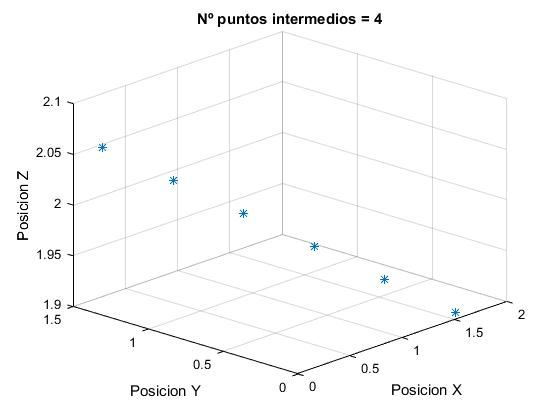
\includegraphics[width=.4\textwidth]{Lineal_4puntos} \hspace{0.25cm} 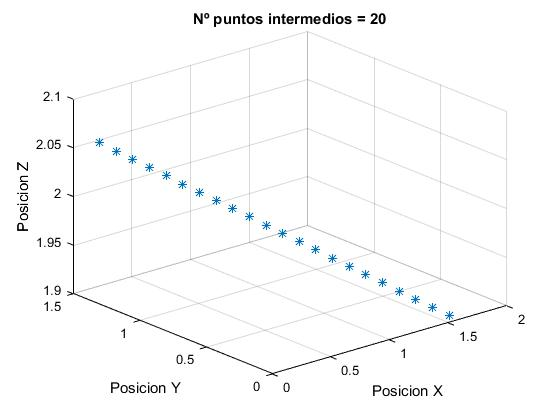
\includegraphics[width=.4\textwidth]{Lineal_20puntos}
		\caption{Generador Trayectorias lineal}
		\end{figure}

\end{itemize}

\begin{itemize}
	\item \textsc{Generador de trayectorias circular}\\

	El generador de trayectorias circulares es similar al generador de trayectorias lineal, excepto por el cálculo de la trayectoria en sí, es decir, una vez obtenidos los puntos que definen la trayectoria, se realizan los mismos cálculos para la obtención de las posiciones, velocidades y aceleraciones articulares. Se empleará también el método heurístico para definir las velocidades de paso.\\

	Para empezar, se deben introducir 3 puntos, a diferencia de los generadores lineales, que definirán la curva como punto inicial($P_1$), punto intermedio($P_2$) y punto final ($P_3$). Tras ello, se calculara el centro de la circunferencia.\\

	Primero se calcula el vector unitario perpendicular al plano definido por la circunferencia:
	\begin{center}
	$v_1=(P_2-P_1)\wedge(P_3-P_1)$\\
	$v_1=\frac{v_1}{||v_1||}$\\
	\end{center}

	Una vez obtenido dicho vector, se pasará al cálculo del centro de la circunferencia($P_0$), lo cual se realiza con un sistema de 3 ecuaciones que se resuelve de forma matricial e imponiendo que se cumplan las siguientes relaciones entre vectores (puede haber más de un sistema de ecuaciones que lleve a la resolución del problema):

	\begin{itemize}
		\item El producto escalar entre el vector $v_1$ y el vector definido por $P_0-P_1$ ha de ser nulo.\\
		\item El producto escalar entre el vector $P_0-\frac{P_2+P_1}{2}$ y el vector $P_2-P_1$ ha de ser nulo.\\
		\item El producto escalar entre el vector $P_0-\frac{P_3+P_1}{2}$ y el vector $P_3-P_1$ ha de ser nulo.\\
	\end{itemize}

	Una vez definidas las ecuaciones se ha de obtener el sistema de ecuaciones que verifique que:\\
	\begin{equation}
		P_0=A|B
	\end{equation}

	Realizando las operaciones pertinentes y despejando se pueden obtener las matrices A y B como:\\
	\begin{equation}
		A=
		\begin{bmatrix}
			v_1(1) & v_1(2) & v_1(3)\\
			P_2(1)-P_1(1) & P_2(2)-P_1(2) & P_2(3)-P_1(3)\\
			P_3(1)-P_1(1) & P_3(2)-P_1(2) & P_3(3)-P_1(3)\\
		\end{bmatrix}
	\end{equation}

\begin{equation}
		B=
		\begin{bmatrix}
			P_1(1)v_1(1)+P_1(2)v_1(2)+P_1(3)v_1(3)\\
			((P_2(1)+P_1(1))\frac{P_2(1)-P_1(1)}{2} + ((P_2(2)+P_1(2))\frac{P_2(2)-P_1(2)}{2}+((P_2(3)+P_1(3))\frac{P_2(3)-P_1(3)}{2} \\
			((P_3(1)+P_1(1))\frac{P_3(1)-P_1(1)}{2} + ((P_3(2)+P_1(2))\frac{P_3(2)-P_1(2)}{2} + ((P_3(3)+P_1(3))\frac{P_3(3)-P_1(3)}{2}\\
		\end{bmatrix}
	\end{equation}

	Una vez hallado el centro de la circunferencia, $P_0$, se debe proceder a calcular los puntos solicitados al principio del algoritmo.\\ Para ello se necesitará definir los siguientes vectores:
	\begin{equation}
		v_2=\frac{P_1-P_0}{||(P_1-P_0)||} \hspace{2cm} v_3=-\frac{v_2 \wedge v_1}{||(v_2 \wedge v_1)||}
	\end{equation}
	que serán, respectivamente, el vector unitario que va desde el centro de la circunferencia al punto $P_1$ y el vector unitario perpendicular al plano definido por $v_1$ y $v_2$ con origen en $P_1$ y sentido de la trayectoria. Con estos dos vectores, el pseudocódigo implementado para calcular los puntos que componen la trayectoria se muestra a continuación:
	\begin{center}
		$g=\frac{P_3-P_0}{||(P_3-P_0)||}$\\
		$cos_g=(v_2 \cdot g)$\\
		$sin_g=||v_2 \wedge g||$\\
		$\rho_{fin}=2\pi-atan2(sin_g,cos_g)$\\
		$\rho=linspace(0,\rho_{fin},num_{ptos})$\\
		$P=repmat(P_0,1,prod(size(\rho))+R(v_2cos(rho)+v_3sin(rho))$\\
	\end{center}

	Siendo $\rho_{fin}$ el ángulo de la posición final de la trayectoria con respecto a la posición inicial, $\rho$ el vector de N puntos de valores de ángulos desde 0 hasta el ángulo de la posición final, $R$ el radio del arco de circunferencia calculado como $R=||P_1-P_0||$, y $P$ la matriz de posiciones correspondientes a los puntos equidistantes a lo largo de la trayectoria.\\

	Una vez realizados estos pasos ya se puede pasar al cálculo de los valores de las variables articulares para las posiciones calculadas como se ha hecho anteriormente en el generador de trayectorias lineal.\\

	Los resultados obtenidos para una trayectoria específica y un valor de 100 puntos a calcular se mostrarán a continuación.
	\begin{figure}[h!]
	\centering
	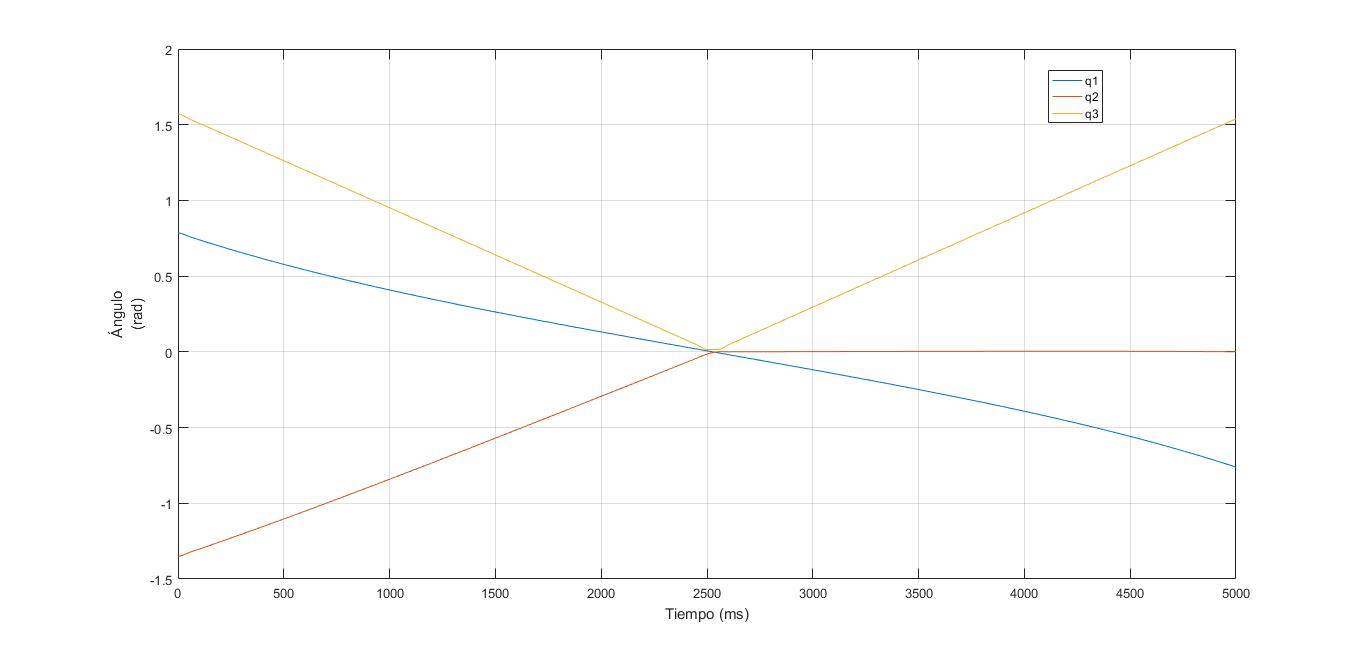
\includegraphics[width=.7\textwidth]{GDT_C_articulares}
	\caption{Valores de las variables articulares}
	\end{figure}

\newpage
Tras ello, la trayectoria ejemplo que podría seguirse en el plano XYZ será:
	\begin{figure}[h!]
	\centering
	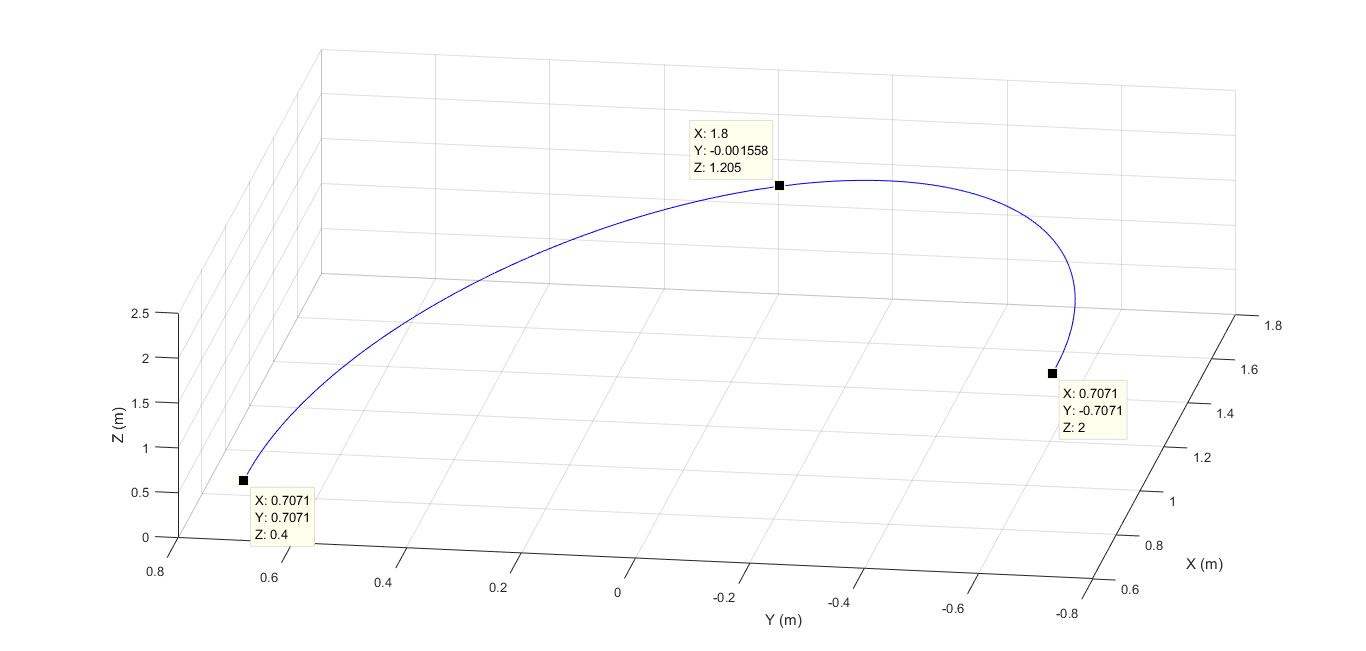
\includegraphics[width=.8\textwidth]{GDT_C_efector}
	\caption{Posición del efector final}
	\end{figure}




\end{itemize}


\subsection{Interpoladores}
Una vez obtenidos estos puntos de referencia, echaremos mano de las herramientas cedidas del análisis cinemático, ya que, se hace uso
del \textit{Modelo Cinematico Inverso}, para la obtención de los puntos de la trayectoria, representadas en el espacio de trabajo
articular del robot.\\


Una vez llegadas aquí, ya tenemos un numero de referencias articulares , que puede conllevar a un control punto a punto;
en nuestro caso, deberemos realizar un linealización de los puntos ya que debemos ser capaces de generar referencias a nuestro sistema
de forma continua. A continuación se tratara el interpolador utilizado.

	\begin{itemize}
		\item SPLINE CÚBICO.\\
		Este interpolador implementa un polinomio de 3º para dar continuidad de la trayectoria de puntos que se les entrege del
		generador pertinente, de la forma:
		\begin{center}
			\begin{equation}
				q(t)= a + b (t-t_{i}) +c (t-t_{i})^{2} + d (t-t_{i})^{3} \hspace{0.75cm};\hspace{0.75cm} t_{i}<t<t_{i+1}
			\end{equation}
			\begin{itemize}
				\item $a = q_{i} $
				\item $b = \dot{q_{i}} $
				\item $c= \frac{3}{T^{2}}(q_{i+1}-q_{i})-\frac{1}{T}(\dot{q}_{i+1}+2\dot{q}_{i})$
				\item $d= -\frac{2}{T^{3}}(q_{i+1}-q_{i})-\frac{1}{T^{2}}(\dot{q}_{i+1}+\dot{q}_{i})$
				\item $T=t_{i+1}-t_{1}$
			\end{itemize}
		\end{center}
		El trabajo matricial de esta ecuación en el espacio articular permite obtener tantos
		polinomios como tramos en la trayectoria sean exigidas por el número de puntos intermedios; pero, para ello debemos asignar valores a
		los parámetros \textit{a, b, c y d}; para estos que contengan parámetros de velocidad, se utilizará
		el método heurístico para la asignación de velocidades articulares.\\

		Le método Heurístico se basta con el análisis de la variación de las posiciones
		articulares de las muestras para asignar una velocidad de la articulación igual a cero, en el caso de que se varíe la
		dirección del movimiento; y una media entre ambas velocidades, si se aportan a la misma dirección de giro. Véase: \\

		\[
		\dot{q}_{i}= \left\{ \begin{array}{ll}
			0 & \textrm{si signo $(q_{i}-q_{i-1})$ $\neq$ signo $(q_{i+1}- q_{i})$} \\
			\frac{(q_{i+1}- q_{i})+(q_{i}-q_{i-1})}{2T} & \textrm{si signo $(q_{i}-q_{i-1})$ = signo $(q_{i+1}- q_{i})$}

		\end{array}\right.
		\]


	\end{itemize}




	\subsection{Pruebas y conclusiones}
	\begin{itemize}
		\item Objetivos: \\
		Ser capaces de que nuestro modelo de brazo manipulador ejecute ordenes de movimientos basados en trayectorias.\\

		\item Necesidad para el trabajo: \\
		Generar trayectorias de referencia en el espacio articular de nuestro modelo brazo manipulador.\\

		\item ¿Como lo hacemos? \\ 
		Herramientas matemáticas. que traduzcan las funcionalidades de la Orden de movimiento. \\ 
		Análisis Cinemático previo con el que poder trasladar las ordenes del espacio cartesiano, al articular del robot.
		Generar Señal de referencia: Aqui asignamos las características de la señal de referencia; asegurar condiciones 
		especificas de velocidad y aceleraciones, además de la continuidad en las consignas de referencia, apoyados en algoritmos
		de interpolación. \\ 

		\begin{figure}[h!]
			\centering
			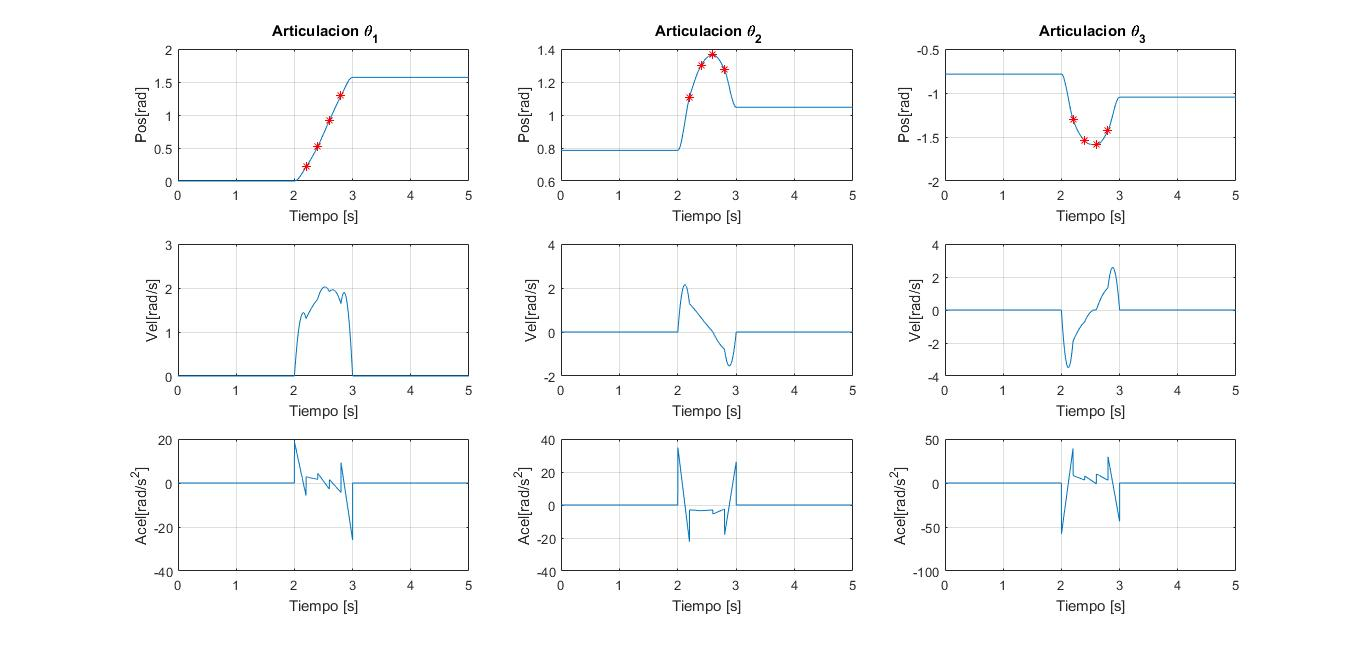
\includegraphics[width=.4\textwidth]{GeneradorTrayLineal}
			\caption{Salida del Control Cinemático con Generador Lineal, e Interpolador cúbico}
		\end{figure}

		Una vez conseguidas estas referencias, y al no poder sen entregadas, como intensidades que varien de forma continua a los motores
		de nuestro modelo de robot, es necesaria la adicion de Mantenedores de Orden Cero, \textit{ZoH}, para ajustar la señal a escalones
		de referencias, que puedan ser referencias reales a nuestro modelo de robot en intensidades.

	
		\begin{figure}[h!]
			\centering
			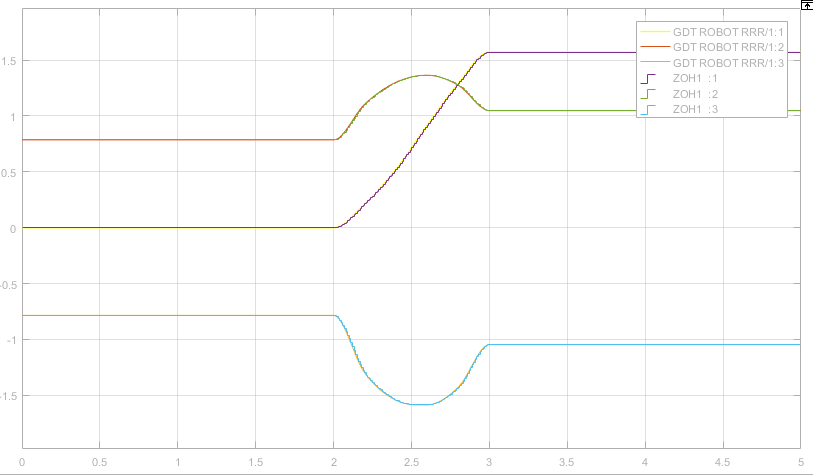
\includegraphics[width=.4\textwidth]{ZoHComparativa} \hspace{0.2cm} 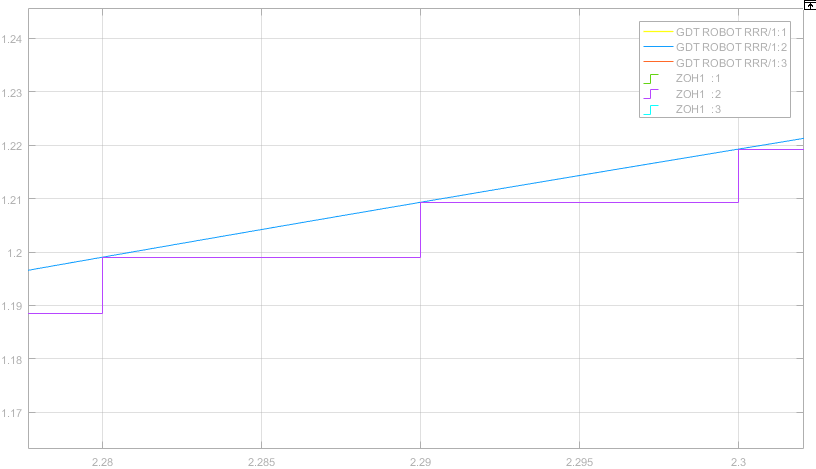
\includegraphics[width=.4\textwidth]{ZoHComparativaDetalle}
			\caption{Referencia Generada Vs Referencia Entregada al Modelo}
		\end{figure}




	\end{itemize}
